% Options for packages loaded elsewhere
\PassOptionsToPackage{unicode}{hyperref}
\PassOptionsToPackage{hyphens}{url}
%
\documentclass[
]{article}
\usepackage{amsmath,amssymb}
\usepackage{iftex}
\ifPDFTeX
  \usepackage[T1]{fontenc}
  \usepackage[utf8]{inputenc}
  \usepackage{textcomp} % provide euro and other symbols
\else % if luatex or xetex
  \usepackage{unicode-math} % this also loads fontspec
  \defaultfontfeatures{Scale=MatchLowercase}
  \defaultfontfeatures[\rmfamily]{Ligatures=TeX,Scale=1}
\fi
\usepackage{lmodern}
\ifPDFTeX\else
  % xetex/luatex font selection
\fi
% Use upquote if available, for straight quotes in verbatim environments
\IfFileExists{upquote.sty}{\usepackage{upquote}}{}
\IfFileExists{microtype.sty}{% use microtype if available
  \usepackage[]{microtype}
  \UseMicrotypeSet[protrusion]{basicmath} % disable protrusion for tt fonts
}{}
\makeatletter
\@ifundefined{KOMAClassName}{% if non-KOMA class
  \IfFileExists{parskip.sty}{%
    \usepackage{parskip}
  }{% else
    \setlength{\parindent}{0pt}
    \setlength{\parskip}{6pt plus 2pt minus 1pt}}
}{% if KOMA class
  \KOMAoptions{parskip=half}}
\makeatother
\usepackage{xcolor}
\usepackage[margin=1in]{geometry}
\usepackage{color}
\usepackage{fancyvrb}
\newcommand{\VerbBar}{|}
\newcommand{\VERB}{\Verb[commandchars=\\\{\}]}
\DefineVerbatimEnvironment{Highlighting}{Verbatim}{commandchars=\\\{\}}
% Add ',fontsize=\small' for more characters per line
\usepackage{framed}
\definecolor{shadecolor}{RGB}{248,248,248}
\newenvironment{Shaded}{\begin{snugshade}}{\end{snugshade}}
\newcommand{\AlertTok}[1]{\textcolor[rgb]{0.94,0.16,0.16}{#1}}
\newcommand{\AnnotationTok}[1]{\textcolor[rgb]{0.56,0.35,0.01}{\textbf{\textit{#1}}}}
\newcommand{\AttributeTok}[1]{\textcolor[rgb]{0.13,0.29,0.53}{#1}}
\newcommand{\BaseNTok}[1]{\textcolor[rgb]{0.00,0.00,0.81}{#1}}
\newcommand{\BuiltInTok}[1]{#1}
\newcommand{\CharTok}[1]{\textcolor[rgb]{0.31,0.60,0.02}{#1}}
\newcommand{\CommentTok}[1]{\textcolor[rgb]{0.56,0.35,0.01}{\textit{#1}}}
\newcommand{\CommentVarTok}[1]{\textcolor[rgb]{0.56,0.35,0.01}{\textbf{\textit{#1}}}}
\newcommand{\ConstantTok}[1]{\textcolor[rgb]{0.56,0.35,0.01}{#1}}
\newcommand{\ControlFlowTok}[1]{\textcolor[rgb]{0.13,0.29,0.53}{\textbf{#1}}}
\newcommand{\DataTypeTok}[1]{\textcolor[rgb]{0.13,0.29,0.53}{#1}}
\newcommand{\DecValTok}[1]{\textcolor[rgb]{0.00,0.00,0.81}{#1}}
\newcommand{\DocumentationTok}[1]{\textcolor[rgb]{0.56,0.35,0.01}{\textbf{\textit{#1}}}}
\newcommand{\ErrorTok}[1]{\textcolor[rgb]{0.64,0.00,0.00}{\textbf{#1}}}
\newcommand{\ExtensionTok}[1]{#1}
\newcommand{\FloatTok}[1]{\textcolor[rgb]{0.00,0.00,0.81}{#1}}
\newcommand{\FunctionTok}[1]{\textcolor[rgb]{0.13,0.29,0.53}{\textbf{#1}}}
\newcommand{\ImportTok}[1]{#1}
\newcommand{\InformationTok}[1]{\textcolor[rgb]{0.56,0.35,0.01}{\textbf{\textit{#1}}}}
\newcommand{\KeywordTok}[1]{\textcolor[rgb]{0.13,0.29,0.53}{\textbf{#1}}}
\newcommand{\NormalTok}[1]{#1}
\newcommand{\OperatorTok}[1]{\textcolor[rgb]{0.81,0.36,0.00}{\textbf{#1}}}
\newcommand{\OtherTok}[1]{\textcolor[rgb]{0.56,0.35,0.01}{#1}}
\newcommand{\PreprocessorTok}[1]{\textcolor[rgb]{0.56,0.35,0.01}{\textit{#1}}}
\newcommand{\RegionMarkerTok}[1]{#1}
\newcommand{\SpecialCharTok}[1]{\textcolor[rgb]{0.81,0.36,0.00}{\textbf{#1}}}
\newcommand{\SpecialStringTok}[1]{\textcolor[rgb]{0.31,0.60,0.02}{#1}}
\newcommand{\StringTok}[1]{\textcolor[rgb]{0.31,0.60,0.02}{#1}}
\newcommand{\VariableTok}[1]{\textcolor[rgb]{0.00,0.00,0.00}{#1}}
\newcommand{\VerbatimStringTok}[1]{\textcolor[rgb]{0.31,0.60,0.02}{#1}}
\newcommand{\WarningTok}[1]{\textcolor[rgb]{0.56,0.35,0.01}{\textbf{\textit{#1}}}}
\usepackage{graphicx}
\makeatletter
\newsavebox\pandoc@box
\newcommand*\pandocbounded[1]{% scales image to fit in text height/width
  \sbox\pandoc@box{#1}%
  \Gscale@div\@tempa{\textheight}{\dimexpr\ht\pandoc@box+\dp\pandoc@box\relax}%
  \Gscale@div\@tempb{\linewidth}{\wd\pandoc@box}%
  \ifdim\@tempb\p@<\@tempa\p@\let\@tempa\@tempb\fi% select the smaller of both
  \ifdim\@tempa\p@<\p@\scalebox{\@tempa}{\usebox\pandoc@box}%
  \else\usebox{\pandoc@box}%
  \fi%
}
% Set default figure placement to htbp
\def\fps@figure{htbp}
\makeatother
\setlength{\emergencystretch}{3em} % prevent overfull lines
\providecommand{\tightlist}{%
  \setlength{\itemsep}{0pt}\setlength{\parskip}{0pt}}
\setcounter{secnumdepth}{-\maxdimen} % remove section numbering
\renewcommand{\contentsname}{Índice}
\usepackage{booktabs}
\usepackage{longtable}
\usepackage{array}
\usepackage{multirow}
\usepackage{wrapfig}
\usepackage{float}
\usepackage{colortbl}
\usepackage{pdflscape}
\usepackage{tabu}
\usepackage{threeparttable}
\usepackage{threeparttablex}
\usepackage[normalem]{ulem}
\usepackage{makecell}
\usepackage{xcolor}
\usepackage{bookmark}
\IfFileExists{xurl.sty}{\usepackage{xurl}}{} % add URL line breaks if available
\urlstyle{same}
\hypersetup{
  pdftitle={ANALISIS EXPLORATORIO 1 CONCESIONARIO DE AUTOS},
  pdfauthor={Alejandra Cifuentes / Giovanny Porras},
  hidelinks,
  pdfcreator={LaTeX via pandoc}}

\title{ANALISIS EXPLORATORIO 1 CONCESIONARIO DE AUTOS}
\author{Alejandra Cifuentes / Giovanny Porras}
\date{2025-05-24}

\begin{document}
\maketitle

{
\setcounter{tocdepth}{2}
\tableofcontents
}
\subsection{2 Exploracion de datos}\label{exploracion-de-datos}

\begin{enumerate}
\def\labelenumi{\alph{enumi}.}
\tightlist
\item
  Descargar el archivo TABLA\_TALLER.xlsx
\item
  Cargar el archivo de datos en RStudio
\end{enumerate}

\textbf{Rta:} Carga de datos inicial

\begin{Shaded}
\begin{Highlighting}[]
\CommentTok{\#datos\_base \textless{}{-} read\_excel("D:/MaestriaAnalitica/BasesAnalitica/gitRepository/Proyecto{-}02{-}Autos/BASE/t1fe{-}tabla\_taller.xlsx")}
\NormalTok{datos\_base }\OtherTok{\textless{}{-}} \FunctionTok{read\_excel}\NormalTok{(}\StringTok{"C:/Users/PC/Documents/ANALITICA/analitics01Cars/BASE/t1fe{-}tabla\_taller.xlsx"}\NormalTok{)}
\FunctionTok{kable}\NormalTok{(}\FunctionTok{head}\NormalTok{(datos\_base, }\DecValTok{10}\NormalTok{,  }\AttributeTok{caption =} \StringTok{"Datos iniciales"}\NormalTok{), }\AttributeTok{format =} \StringTok{"latex"}\NormalTok{, }\AttributeTok{booktabs =} \ConstantTok{TRUE}\NormalTok{) }\SpecialCharTok{\%\textgreater{}\%} 
  \FunctionTok{kable\_styling}\NormalTok{(}\AttributeTok{latex\_options =} \FunctionTok{c}\NormalTok{(}\StringTok{"scale\_down"}\NormalTok{, }\StringTok{"hold\_position"}\NormalTok{))}
\end{Highlighting}
\end{Shaded}

\begin{table}[!h]
\centering
\resizebox{\ifdim\width>\linewidth\linewidth\else\width\fi}{!}{
\begin{tabular}{lllllllrl}
\toprule
PERSONA & EDAD & SEXO & ESTATURA & NIVEL ESCOLAR & MARCA DE AUTO & NUMERO DE HIJOS & SALARIO & MASCOTA\\
\midrule
NA & NA & NA & NA & NA & NA & NA & NA & NA\\
NA & NA & NA & NA & NA & NA & NA & NA & NA\\
PERSONA 1 & 21 & M & 1.54 & MAESTRÍA & AUDI & 0 & 1200000 & SI\\
PERSONA 2 & 26 & F & 1.55 & PROFESIONAL & RENAULT & 5 & 1250000 & NO\\
PERSONA 3 & 30 & F & 1.6 & DOCTORADO & BMW & 2 & 900000 & NO\\
\addlinespace
PERSONA 4 & 31 & f & 1.7 & PROFESIONAL & RENAULT & 2 & 800000 & NO\\
PERSONA 5 & 35 & M & 1.71 & MAESTRÍA & AUDI & 1 & 950000 & NO\\
PERSONA 6 & 65 & M & 1.8 & MAESTRÍA & AUDI & 1 & 2000000 & SI\\
PERSONA 7 & 45 & M & 1.54 & MAESTRÍA & BMW & 1 & 2500000 & NO\\
PERSONA 8 & 42 & F & 1.52 & PROFESIONAL & RENAULT & 1 & 3500000 & SI\\
\bottomrule
\end{tabular}}
\end{table}

\begin{enumerate}
\def\labelenumi{\alph{enumi}.}
\setcounter{enumi}{2}
\tightlist
\item
  Describir brevemente la estructura del conjunto de datos: ¿Cuantos
  clientes estan registrados y que variables incluyen?
\end{enumerate}

\begin{Shaded}
\begin{Highlighting}[]
\NormalTok{no\_datos\_persona }\OtherTok{\textless{}{-}}\NormalTok{ datos\_base }\SpecialCharTok{\%\textgreater{}\%}
  \FunctionTok{filter}\NormalTok{(}\FunctionTok{grepl}\NormalTok{(}\StringTok{"PERSONA"}\NormalTok{, PERSONA)) }\SpecialCharTok{\%\textgreater{}\%}
  \FunctionTok{count}\NormalTok{()}

\NormalTok{cabeceras\_datos }\OtherTok{\textless{}{-}} \FunctionTok{names}\NormalTok{(datos\_base)}
\end{Highlighting}
\end{Shaded}

\textbf{Rta:} El conjunto de datos tiene 60 clientes registrados e
incluyen las varibles PERSONA, EDAD, SEXO, ESTATURA, NIVEL ESCOLAR,
MARCA DE AUTO, NUMERO DE HIJOS, SALARIO, MASCOTA .

\begin{enumerate}
\def\labelenumi{\alph{enumi}.}
\setcounter{enumi}{3}
\tightlist
\item
  Realizar una exploracion rapida utilizando funciones como head(),
  tail(), str(), summary(), \textbf{Rta:} Los ultimos valores son (tail)
\end{enumerate}

\begin{Shaded}
\begin{Highlighting}[]
\NormalTok{ultimos\_datos }\OtherTok{\textless{}{-}} \FunctionTok{tail}\NormalTok{(datos\_base)}
\FunctionTok{kable}\NormalTok{(}\FunctionTok{head}\NormalTok{(ultimos\_datos, }\DecValTok{10}\NormalTok{, }\AttributeTok{caption =} \StringTok{"Datos ultima posicion"}\NormalTok{), }\AttributeTok{format =} \StringTok{"latex"}\NormalTok{, }\AttributeTok{booktabs =} \ConstantTok{TRUE}\NormalTok{) }\SpecialCharTok{\%\textgreater{}\%}\FunctionTok{kable\_styling}\NormalTok{(}\AttributeTok{latex\_options =} \FunctionTok{c}\NormalTok{(}\StringTok{"scale\_down"}\NormalTok{, }\StringTok{"hold\_position"}\NormalTok{))}
\end{Highlighting}
\end{Shaded}

\begin{table}[!h]
\centering
\resizebox{\ifdim\width>\linewidth\linewidth\else\width\fi}{!}{
\begin{tabular}{lllllllrl}
\toprule
PERSONA & EDAD & SEXO & ESTATURA & NIVEL ESCOLAR & MARCA DE AUTO & NUMERO DE HIJOS & SALARIO & MASCOTA\\
\midrule
PERSONA 55 & 30 & F & 1.54 & MAESTRÍA & CHEVROLET & 2 & 2400000 & SI\\
PERSONA 56 & 39 & M & 1.58 & MAESTRÍA & AUDI & 1 & 2600000 & NO\\
PERSONA 57 & 34 & F & 1.6 & DOCTORADO & BMW & 1 & 3500000 & SI\\
PERSONA 58 & 24 & f & 1.7 & PROFESIONAL & RENAULT & 3 & 800000 & SI\\
PERSONA 59 & 20 & M & 1.71 & MAESTRÍA & AUDI & 0 & 850000 & NO\\
\addlinespace
PERSONA 60 & 10 & M & 1.8 & PROFESIONAL & AUDI & 0 & 1000000 & NO\\
\bottomrule
\end{tabular}}
\end{table}

\textbf{Funciones adicionales:}

\begin{Shaded}
\begin{Highlighting}[]
\CommentTok{\#print(str(datos\_base))}
\CommentTok{\#print(dim(datos\_base))}
\CommentTok{\#print(colnames(datos\_base))}
\FunctionTok{print}\NormalTok{(}\FunctionTok{summary}\NormalTok{(datos\_base))}
\end{Highlighting}
\end{Shaded}

\begin{verbatim}
##    PERSONA              EDAD               SEXO             ESTATURA        
##  Length:62          Length:62          Length:62          Length:62         
##  Class :character   Class :character   Class :character   Class :character  
##  Mode  :character   Mode  :character   Mode  :character   Mode  :character  
##                                                                             
##                                                                             
##                                                                             
##                                                                             
##  NIVEL ESCOLAR      MARCA DE AUTO      NUMERO DE HIJOS       SALARIO       
##  Length:62          Length:62          Length:62          Min.   : 800000  
##  Class :character   Class :character   Class :character   1st Qu.:2000000  
##  Mode  :character   Mode  :character   Mode  :character   Median :3450000  
##                                                           Mean   :3286667  
##                                                           3rd Qu.:4700000  
##                                                           Max.   :6500000  
##                                                           NA's   :2        
##    MASCOTA         
##  Length:62         
##  Class :character  
##  Mode  :character  
##                    
##                    
##                    
## 
\end{verbatim}

\begin{enumerate}
\def\labelenumi{\alph{enumi}.}
\setcounter{enumi}{4}
\tightlist
\item
  Identificar si hay datos faltantes y cuantificar cuantos son en total
  y por variable
\end{enumerate}

\begin{Shaded}
\begin{Highlighting}[]
\CommentTok{\#is.na(datos\_base)}
\NormalTok{total\_na }\OtherTok{=}\NormalTok{ datos\_base }\SpecialCharTok{\%\textgreater{}\%}\NormalTok{ is.na }\SpecialCharTok{\%\textgreater{}\%} \FunctionTok{sum}\NormalTok{()  }
\CommentTok{\#Contar NA por columna(variable) }
\NormalTok{na\_por\_columna }\OtherTok{\textless{}{-}} \FunctionTok{colSums}\NormalTok{(}\FunctionTok{is.na}\NormalTok{(datos\_base))}
\NormalTok{tabla\_na }\OtherTok{\textless{}{-}} \FunctionTok{data.frame}\NormalTok{(}
   \AttributeTok{Variable =} \FunctionTok{names}\NormalTok{(na\_por\_columna), }
   \AttributeTok{total\_na =} \FunctionTok{as.vector}\NormalTok{(na\_por\_columna) }
\NormalTok{)}

\CommentTok{\#Contar NA total }
\CommentTok{\#rowSums(is.na(datos\_base))}

\CommentTok{\#Impresion de tabla }
\CommentTok{\#kable(tabla\_na, caption = "Variables faltantes por cuantificar")  \%\textgreater{}\%}
\CommentTok{\#  kable\_styling(full\_width = FALSE, position = "left")}
\end{Highlighting}
\end{Shaded}

\textbf{Rta}: - El numero de total de datos faltantes es \textbf{24} y
por variable son los siguientes:

\begin{longtable}[l]{lr}
\caption{\label{tab:tabla_variables_na}Variables faltantes por cuantificar}\\
\toprule
Variable & total\_na\\
\midrule
PERSONA & 2\\
EDAD & 2\\
SEXO & 3\\
ESTATURA & 2\\
NIVEL ESCOLAR & 3\\
\addlinespace
MARCA DE AUTO & 4\\
NUMERO DE HIJOS & 3\\
SALARIO & 2\\
MASCOTA & 3\\
\bottomrule
\end{longtable}

\begin{itemize}
\tightlist
\item
  Analisis: Hay problemas de datos en todas las variables sera
  importante discriminar cada caso
\end{itemize}

\begin{enumerate}
\def\labelenumi{\alph{enumi}.}
\setcounter{enumi}{5}
\tightlist
\item
  Comentar sobre los posibles problemas en los datos:
\end{enumerate}

\textbf{Filas vacías al inicio del archivo:} - Las dos primeras filas
están vacías o no contienen datos válidos.

\textbf{Inconsistencias categóricas:}

\begin{itemize}
\tightlist
\item
  Variabilidad en la codificación de la variable SEXO, con valores como
  f, mujer, hombre, nan o minúsculas inconsistentes.
\item
  Formatos no estandarizados en NIVEL ESCOLAR, como el uso de PhD en
  lugar de DOCTORADO.
\item
  Uso de minúsculas en valores de MARCA DE AUTO, como renault.
\end{itemize}

\textbf{Valores faltantes:}

\begin{itemize}
\tightlist
\item
  Algunas filas tienen múltiples variables vacías, como en el caso de la
  PERSONA 24.
\end{itemize}

\textbf{Valores extremos o anómalos (outliers):}

\begin{itemize}
\tightlist
\item
  PERSONA 31: valor de ESTATURA = 3.45 m, fuera del rango fisiológico
  normal.
\item
  PERSONA 33: valor de NUMERO DE HIJOS = 54, ampliamente fuera del
  promedio observado (3.03).
\end{itemize}

\newpage

\subsection{3 Análisis de la variable Marca ``Marca de
auto''.}\label{anuxe1lisis-de-la-variable-marca-marca-de-auto.}

\begin{enumerate}
\def\labelenumi{\alph{enumi}.}
\tightlist
\item
  Evaluar la variable \textbf{``MARCA DE AUTO''} y determinar si hay
  faltantes.
\end{enumerate}

\begin{Shaded}
\begin{Highlighting}[]
 \CommentTok{\#datos\_base$\textasciigrave{}MARCA DE AUTO\textasciigrave{}(is.na)}
 \CommentTok{\#(is.na(datos\_base$\textasciigrave{}MARCA DE AUTO\textasciigrave{}))}
\NormalTok{ data\_na\_marca\_autos }\OtherTok{\textless{}{-}} \FunctionTok{sum}\NormalTok{(}\FunctionTok{is.na}\NormalTok{(datos\_base}\SpecialCharTok{$}\StringTok{\textasciigrave{}}\AttributeTok{MARCA DE AUTO}\StringTok{\textasciigrave{}}\NormalTok{))}
\end{Highlighting}
\end{Shaded}

\textbf{Rta:} Se tratan datos faltantes y se encuentran un total de
\textbf{4}; se realiza tratamiento de datos remplazando los
``na''/``NA'' a ``NO\_MANEJA'', se convierte todo mayúsculas.

\begin{Shaded}
\begin{Highlighting}[]
 \FunctionTok{Sys.setlocale}\NormalTok{(}\StringTok{"LC\_ALL"}\NormalTok{, }\StringTok{"Spanish\_Colombia.UTF{-}8"}\NormalTok{)}
\end{Highlighting}
\end{Shaded}

\begin{verbatim}
## [1] "LC_COLLATE=Spanish_Colombia.utf8;LC_CTYPE=Spanish_Colombia.utf8;LC_MONETARY=Spanish_Colombia.utf8;LC_NUMERIC=C;LC_TIME=Spanish_Colombia.utf8"
\end{verbatim}

\begin{Shaded}
\begin{Highlighting}[]
 \CommentTok{\#Eliminar columna 1, 2 }
\NormalTok{ datos\_base }\OtherTok{\textless{}{-}}\NormalTok{ datos\_base[}\SpecialCharTok{{-}}\FunctionTok{c}\NormalTok{(}\DecValTok{1}\NormalTok{,}\DecValTok{2}\NormalTok{), ]}
 \CommentTok{\#Datos Eliminados}
 \CommentTok{\#print(datos\_base)}
\NormalTok{ na\_marca\_autos }\OtherTok{\textless{}{-}} \FunctionTok{sum}\NormalTok{(}\FunctionTok{is.na}\NormalTok{(datos\_base}\SpecialCharTok{$}\StringTok{\textasciigrave{}}\AttributeTok{MARCA DE AUTO}\StringTok{\textasciigrave{}}\NormalTok{)) }
 \CommentTok{\# PERSONA 13, 32, 49, NA y datos vacios }
\NormalTok{ datos\_base}\SpecialCharTok{$}\StringTok{\textasciigrave{}}\AttributeTok{MARCA DE AUTO}\StringTok{\textasciigrave{}}\NormalTok{[}\FunctionTok{is.na}\NormalTok{(datos\_base}\SpecialCharTok{$}\StringTok{\textasciigrave{}}\AttributeTok{MARCA DE AUTO}\StringTok{\textasciigrave{}}\NormalTok{) }\SpecialCharTok{|}\NormalTok{ datos\_base}\SpecialCharTok{$}\StringTok{\textasciigrave{}}\AttributeTok{MARCA DE AUTO}\StringTok{\textasciigrave{}} \SpecialCharTok{==} \StringTok{"NA"}\NormalTok{] }\OtherTok{\textless{}{-}} \StringTok{"SIN\_CONFIRMAR"}
 \CommentTok{\# PERSONA 39 cambia FOR A FORD }
\NormalTok{ datos\_base}\SpecialCharTok{$}\StringTok{\textasciigrave{}}\AttributeTok{MARCA DE AUTO}\StringTok{\textasciigrave{}}\NormalTok{[ datos\_base}\SpecialCharTok{$}\StringTok{\textasciigrave{}}\AttributeTok{MARCA DE AUTO}\StringTok{\textasciigrave{}} \SpecialCharTok{==} \StringTok{"FOR"}\NormalTok{] }\OtherTok{\textless{}{-}} \StringTok{"FORD"}
 \CommentTok{\# PERSONA 40 cambia BWM A BMW }
\NormalTok{ datos\_base}\SpecialCharTok{$}\StringTok{\textasciigrave{}}\AttributeTok{MARCA DE AUTO}\StringTok{\textasciigrave{}}\NormalTok{[ datos\_base}\SpecialCharTok{$}\StringTok{\textasciigrave{}}\AttributeTok{MARCA DE AUTO}\StringTok{\textasciigrave{}} \SpecialCharTok{==} \StringTok{"BWM"}\NormalTok{] }\OtherTok{\textless{}{-}} \StringTok{"BMW"}
 
 \CommentTok{\#print(datos\_base)}
 \CommentTok{\# PERSONA 36 cambio a mayuscula marca }
\NormalTok{ datos\_base}\SpecialCharTok{$}\StringTok{\textasciigrave{}}\AttributeTok{MARCA DE AUTO}\StringTok{\textasciigrave{}} \OtherTok{\textless{}{-}} \FunctionTok{toupper}\NormalTok{(datos\_base}\SpecialCharTok{$}\StringTok{\textasciigrave{}}\AttributeTok{MARCA DE AUTO}\StringTok{\textasciigrave{}}\NormalTok{)}
 \FunctionTok{print}\NormalTok{(datos\_base)}
\end{Highlighting}
\end{Shaded}

\begin{verbatim}
## # A tibble: 60 x 9
##    PERSONA    EDAD  SEXO  ESTATURA `NIVEL ESCOLAR` `MARCA DE AUTO`
##    <chr>      <chr> <chr> <chr>    <chr>           <chr>          
##  1 PERSONA 1  21    M     1.54     MAESTRÍA        AUDI           
##  2 PERSONA 2  26    F     1.55     PROFESIONAL     RENAULT        
##  3 PERSONA 3  30    F     1.6      DOCTORADO       BMW            
##  4 PERSONA 4  31    f     1.7      PROFESIONAL     RENAULT        
##  5 PERSONA 5  35    M     1.71     MAESTRÍA        AUDI           
##  6 PERSONA 6  65    M     1.8      MAESTRÍA        AUDI           
##  7 PERSONA 7  45    M     1.54     MAESTRÍA        BMW            
##  8 PERSONA 8  42    F     1.52     PROFESIONAL     RENAULT        
##  9 PERSONA 9  52    F     1.51     DOCTORADO       RENAULT        
## 10 PERSONA 10 63    M     1.65     DOCTORADO       RENAULT        
## # i 50 more rows
## # i 3 more variables: `NUMERO DE HIJOS` <chr>, SALARIO <dbl>, MASCOTA <chr>
\end{verbatim}

\begin{enumerate}
\def\labelenumi{\alph{enumi}.}
\setcounter{enumi}{1}
\tightlist
\item
  Crear un tabla de frecuencias para entender la popularidad de las
  diferentes marcas entre los cliente. \textbf{Rta:} En la tabla de
  frecuencias se observa que las marcas más populares son AUDI,
  CHEVROLET, RENAULT y BMW. Los tres usuarios que no tienen la categoría
  ``\,``SIN\_CONFIRMAR''\,'' se identificaron como personas a partir de
  50 años
\end{enumerate}

\begin{Shaded}
\begin{Highlighting}[]
\NormalTok{tabla\_frecuencias\_autos }\OtherTok{\textless{}{-}} \FunctionTok{as.data.frame}\NormalTok{(}\FunctionTok{table}\NormalTok{(datos\_base}\SpecialCharTok{$}\StringTok{\textasciigrave{}}\AttributeTok{MARCA DE AUTO}\StringTok{\textasciigrave{}}\NormalTok{))}
\FunctionTok{names}\NormalTok{(tabla\_frecuencias\_autos) }\OtherTok{\textless{}{-}} \FunctionTok{c}\NormalTok{(}\StringTok{"MARCA DE AUTO"}\NormalTok{, }\StringTok{"Frecuencia"}\NormalTok{)}
\CommentTok{\#Organizar Mayor a menor}
\NormalTok{tabla\_frecuencias\_autos }\OtherTok{\textless{}{-}}\NormalTok{ tabla\_frecuencias\_autos }\SpecialCharTok{\%\textgreater{}\%} \FunctionTok{arrange}\NormalTok{(}\FunctionTok{desc}\NormalTok{(Frecuencia))}
\FunctionTok{print}\NormalTok{(tabla\_frecuencias\_autos)}
\end{Highlighting}
\end{Shaded}

\begin{verbatim}
##   MARCA DE AUTO Frecuencia
## 1          AUDI         13
## 2       RENAULT         13
## 3           BMW         12
## 4     CHEVROLET         12
## 5          FORD          7
## 6 SIN_CONFIRMAR          3
\end{verbatim}

\begin{enumerate}
\def\labelenumi{\alph{enumi}.}
\setcounter{enumi}{2}
\tightlist
\item
  Generar graficos de barras y de tortas para visualizar la distribucion
  de las marcas de autos y proporcionar una interpretacion. \textbf{Rta:
  } Se identifica que las marcas de vehiculos preferidas por los
  clientes del concesionario son \textbf{AUDi} y \textbf{RENAULT}; se
  observa una segmentacion igual por pares entre las entre AUDI/RENAULT
  y CHEVROLET/BMW
\end{enumerate}

\pandocbounded{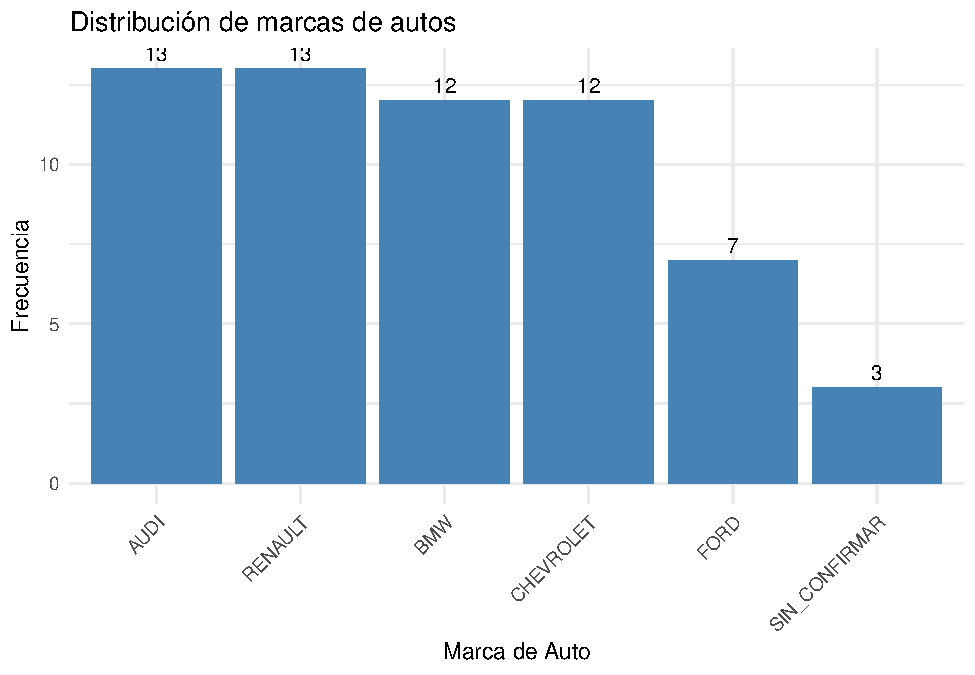
\includegraphics[keepaspectratio]{Reporte01-autors_files/figure-latex/grafico_barras_marcas-1.pdf}}
\textbf{Rta: } La preferencia de vehículos esta distribuida entre 4
marcas que suman 83\% de la muestra, estas cuatro marcas a su vez
representan dos segmentos que se reparten en el mismo porcentaje
21\%/21\% y 20\%/20\%.

\begin{enumerate}
\def\labelenumi{\alph{enumi}.}
\setcounter{enumi}{3}
\tightlist
\item
  Concluir cuál es la marca de auto más popular entre los clientes.
  \textbf{Rta:} Se concluyen que AUDI y RENAULT son las marcas lideres
  con una distribución uniforme en el los clientes del concesionario en
  un porcentaje del 21.7 entre ambas ocupan el 42.4\%.
\end{enumerate}

\begin{Shaded}
\begin{Highlighting}[]
\NormalTok{tabla\_frecuencias\_autos}\SpecialCharTok{$}\NormalTok{Porcentaje }\OtherTok{\textless{}{-}} \FunctionTok{round}\NormalTok{(tabla\_frecuencias\_autos}\SpecialCharTok{$}\NormalTok{Frecuencia}\SpecialCharTok{/}\FunctionTok{sum}\NormalTok{(tabla\_frecuencias\_autos}\SpecialCharTok{$}\NormalTok{Frecuencia)}\SpecialCharTok{*}\DecValTok{100}\NormalTok{, }\DecValTok{1}\NormalTok{)}
\FunctionTok{print}\NormalTok{(tabla\_frecuencias\_autos)}
\end{Highlighting}
\end{Shaded}

\begin{verbatim}
##   MARCA DE AUTO Frecuencia Porcentaje
## 1          AUDI         13       21.7
## 2       RENAULT         13       21.7
## 3           BMW         12       20.0
## 4     CHEVROLET         12       20.0
## 5          FORD          7       11.7
## 6 SIN_CONFIRMAR          3        5.0
\end{verbatim}

\begin{Shaded}
\begin{Highlighting}[]
\NormalTok{tabla\_frecuencias\_autos}\SpecialCharTok{$}\StringTok{\textasciigrave{}}\AttributeTok{MARCA DE AUTO}\StringTok{\textasciigrave{}} \OtherTok{\textless{}{-}} \FunctionTok{factor}\NormalTok{(}
\NormalTok{  tabla\_frecuencias\_autos}\SpecialCharTok{$}\StringTok{\textasciigrave{}}\AttributeTok{MARCA DE AUTO}\StringTok{\textasciigrave{}}\NormalTok{,}
  \AttributeTok{levels =}\NormalTok{ tabla\_frecuencias\_autos}\SpecialCharTok{$}\StringTok{\textasciigrave{}}\AttributeTok{MARCA DE AUTO}\StringTok{\textasciigrave{}}\NormalTok{[}\FunctionTok{order}\NormalTok{(}\SpecialCharTok{{-}}\NormalTok{tabla\_frecuencias\_autos}\SpecialCharTok{$}\NormalTok{Frecuencia)]}
\NormalTok{)}
\CommentTok{\# Crear el grafico circular de MARCAS AUTOS }
\FunctionTok{ggplot}\NormalTok{(tabla\_frecuencias\_autos, }\FunctionTok{aes}\NormalTok{(}\AttributeTok{x =} \StringTok{""}\NormalTok{, }\AttributeTok{y =}\NormalTok{ Frecuencia, }\AttributeTok{fill =} \StringTok{\textasciigrave{}}\AttributeTok{MARCA DE AUTO}\StringTok{\textasciigrave{}}\NormalTok{)) }\SpecialCharTok{+}
  \FunctionTok{geom\_bar}\NormalTok{(}\AttributeTok{stat =} \StringTok{"identity"}\NormalTok{, }\AttributeTok{width =} \DecValTok{1}\NormalTok{) }\SpecialCharTok{+}
  \FunctionTok{coord\_polar}\NormalTok{(}\StringTok{"y"}\NormalTok{, }\AttributeTok{start =} \DecValTok{0}\NormalTok{) }\SpecialCharTok{+}
  \FunctionTok{geom\_text}\NormalTok{(}\FunctionTok{aes}\NormalTok{(}\AttributeTok{label =} \FunctionTok{paste0}\NormalTok{(Porcentaje, }\StringTok{"\%"}\NormalTok{)),}
            \AttributeTok{position =} \FunctionTok{position\_stack}\NormalTok{(}\AttributeTok{vjust =} \FloatTok{0.5}\NormalTok{),}
            \AttributeTok{size =} \DecValTok{4}\NormalTok{,}
            \AttributeTok{color =} \StringTok{"black"}\NormalTok{,}
            \AttributeTok{fontface =} \StringTok{"bold"}\NormalTok{) }\SpecialCharTok{+}
  \FunctionTok{labs}\NormalTok{(}\AttributeTok{title =} \StringTok{"Distribucion Marcas de Autos"}\NormalTok{,}
       \AttributeTok{fill =} \StringTok{"MARCA DE AUTO"}\NormalTok{) }\SpecialCharTok{+}
  \FunctionTok{scale\_fill\_brewer}\NormalTok{(}\AttributeTok{palette =} \StringTok{"Paired"}\NormalTok{) }\SpecialCharTok{+}  \CommentTok{\# Usando paleta predefinida}
  \FunctionTok{theme\_void}\NormalTok{() }\SpecialCharTok{+}
  \FunctionTok{theme}\NormalTok{(}\AttributeTok{legend.position =} \StringTok{"right"}\NormalTok{,}
        \AttributeTok{plot.title =} \FunctionTok{element\_text}\NormalTok{(}\AttributeTok{hjust =} \FloatTok{0.5}\NormalTok{, }\AttributeTok{face =} \StringTok{"bold"}\NormalTok{))}
\end{Highlighting}
\end{Shaded}

\pandocbounded{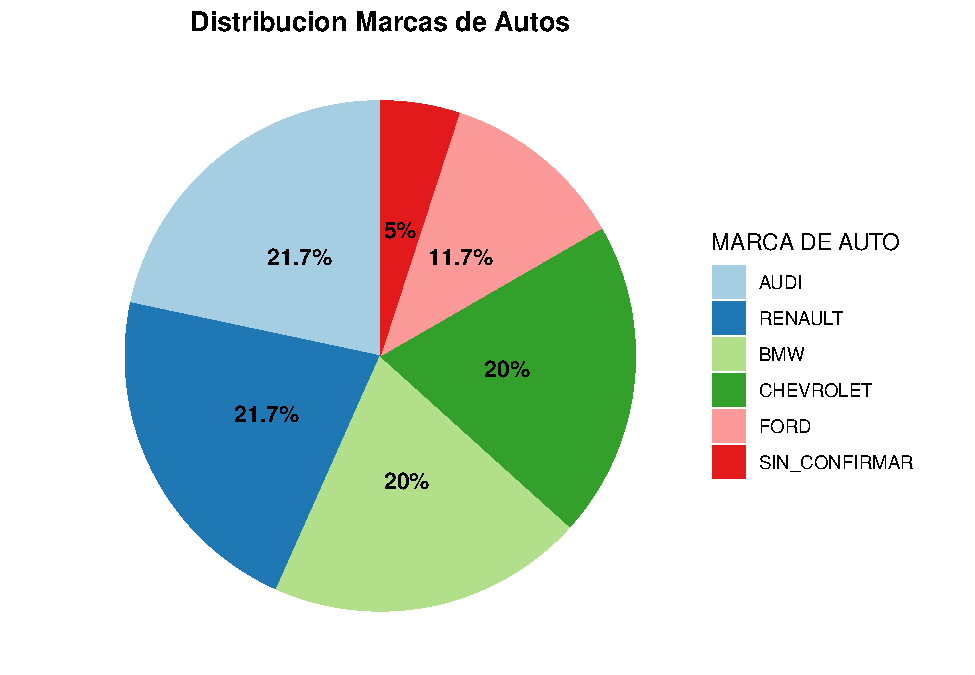
\includegraphics[keepaspectratio]{Reporte01-autors_files/figure-latex/unnamed-chunk-7-1.pdf}}
\newpage

\subsection{5 Análisis de la variable
``Estatura''.}\label{anuxe1lisis-de-la-variable-estatura.}

\begin{enumerate}
\def\labelenumi{\alph{enumi}.}
\item
  Revisar la variable ``ESTATURA'' para asegurar que este correctamente
  importada y limpia. \textbf{Rta:}
\item
  Identificar los datos faltantes o valores inconsistentes. Eliminar
  esos registros. \textbf{Rta:}
\item
  Generar un poligono de frecuencia y una ojiva para analizar la
  distribución de la estatura de los clientes y extraer conclusiones.
  \textbf{Rta:}
\end{enumerate}

\newpage

\subsection{6 Análisis de la variable ``Numero de
hijos''.}\label{anuxe1lisis-de-la-variable-numero-de-hijos.}

\begin{enumerate}
\def\labelenumi{\alph{enumi}.}
\item
  Cambiar el nombre de l varaible a ``n.hijos'' para facilitar su
  manejo. \textbf{Rta:}
\item
  Identificar problemas con los datos y eliminar valores inconsistentes.
  \textbf{Rta:}
\item
  Generar una grafica de barras con colores y analizar que se puede
  concluir sobre el numero de hijos de los clientes. \textbf{Rta:}
\end{enumerate}

\newpage

\subsection{7 Análisis de la variable
``Sexo''.}\label{anuxe1lisis-de-la-variable-sexo.}

\begin{enumerate}
\def\labelenumi{\alph{enumi}.}
\item
  Revisar la consistencia de los datos de la varaible ``SEXO'' y
  realizar correcciones en caso de encontrar valores inusuales o
  inconsistentes. \textbf{Rta:}
\item
  Crea una tabla de frecuencias y extraer conclusiones sobre la
  proporcion de hombres y mujeres en el conjunto de clientes.
  \textbf{Rta:}
\end{enumerate}

\newpage

\subsection{8 Preguntas de
investigación''.}\label{preguntas-de-investigaciuxf3n.}

\begin{enumerate}
\def\labelenumi{\alph{enumi}.}
\setcounter{enumi}{2}
\item
  ¿Cuantos clientes con doctorado ganan mas de 2 millones de pesos?
  \textbf{Rta:}
\item
  ¿Cual es el promedio de salario por cada categoria de variable ``MARCA
  DE AUTO''? \textbf{Rta:}
\end{enumerate}

\end{document}
